\chapter{Experiments}\label{chap:experiments}
In this section we will test the methods discussed in \ref{sec:second}, and evaluate their performance for different models. We want to investigate whether the methods presented in the previous sections actually perform better in a tall data situation than the regular MH algorithm.  \\
The methods we have tested are given in the table below: 

\begin{table}[ht]
    \centering
        \begin{tabular}{|c|c|c|c|c|}
    \hline
    \multicolumn{5}{|c|}{Methods} \\
    \hline
   Model & MH & FlyMC & Bardenet et. al 2014 & Bardenet et al. 2017\\ \hline\hline
        Gaussian & V & V & V &V \\
        Logistic regression &V &V &V &V  \\
        Linear regression &V & V& X& X \\ \hline
    \end{tabular}{}
    \caption{Overview of which models we have tested for the different methods. Here V indicates that the model is tested, and X that it is not.}
    \label{tab:experiment_overview}
\end{table}{}
We will use the number of required likelihood evaluations before convergence of the chain to the invariant distribution to be a measure of a methods performance.
Here, we will use the Gelman-Rubin statistic as a criterion for convergence, and also use the within chain correlation and other criteria to assess the quality of the method. 
\todo{fiks setning}
\texttt{Obviously} the methods presented in the Chapter \ref{chap:method} have fewer likelihood evaluations per iteration, but one can imagine that because of fewer likelihood evaluations, the number of iterations needed to mixing may be larger than for the vanilla MH algorithm. 



\section{Standard normal data}
We simulated standard normal data as shown below and used the different MCMC methods discussed in Chapter \ref{chap:method} to make inference about the model parameters.
\begin{equation*}
    x_n \sim \mathcal{N}\left(\mu,\sigma^2\right)
\end{equation*}
we set $\mu = 0$ and $\sigma^2 = 1$, so that the data $x_{n, n\in \left[1, N\right]}$ were standard normal. 
%\begin{lstlisting}[caption={simulation of standard normal data}, label={lst:sim_normal}]
%set.seed(1234)
%N = 1000
%x = rnorm(N, 0, 1)
%\end{lstlisting}
We simulate samples from the posterior density $p\left(\theta\mid x_1 \cdots x_N\right)$ as described in Algorithm \ref{algo:MH} for the Metropolis-Hastings, Algorithm \ref{algo:firefly} for the Firefly method, Algorithm \ref{algo:conf_sampl} for the confidence sampler, and Algorithm \ref{algo:conf_sampl} with the changes of Step \ref{state:lambda_star}, Step \ref{algo_state:confidence_test} and Step \ref{confidence:accept} as described in Chapter \ref{sec:adap_subsampl}. We have chosen a flat prior for all parameters. In a tall data setting, the prior will have less influence on the resulting posterior than in a setting with less data. However, if one finds it necessary, it is simple to implement all methods with other priors than a flat one. 
We chose to sample $\sigma$ on a log-scale so that both$\mu$ and $\log\sigma$ easily could be sampled from the same distribution.
For the proposal distribution, $g\left(\cdot\mid\theta\right)$ from which the proposed parameter $\theta' = \left(\mu', e^{\left(\log \sigma\right)'}\right)$ were drawn, we chose $\mathcal{N}\left(0, \frac{1}{N}\right)$, with $N$ the total number of data points in the data set . This results in a symmetric proposal distribution for $\mu$ and $\log \sigma$, but unsymmetrical for $\sigma$. We do a transformation of variable from $\log \sigma$ to $\sigma$ to get the correct acceptance probability $\alpha \left(\theta, \theta'\right)$. Thus. for Step \ref{state:accept_reject_MH} in Algorithm \ref{algo:MH} we check whether 
\begin{equation*}
\begin{split}
    &\frac{p\left(\theta' \mid \mathbf{x}\right) \frac{\sqrt{N}}{\sqrt{2\pi}}e^{-\frac{N}{2}\left(\log \sigma -\left(\log\sigma\right)'  \right)^2}\sigma'}{p\left(\theta \mid \mathbf{x}\right) \frac{\sqrt{N}}{\sqrt{2\pi}}e^{-\frac{N}{2}\left( \left(\log\sigma\right)' - \log \sigma \right)^2}\sigma} \\
    &= \frac{p\left(\theta'\mid \mathbf{x}\right) \sigma'}{p\left(\theta\mid \mathbf{x}\right) \sigma} < u
    \end{split}
\end{equation*}
to decide if the $\theta'$ is accepted or rejected. 
Equivalently for Algorithm \ref{algo:firefly}, the acceptance probability $\alpha\left(\theta, \theta'\right)$ in Step \ref{algo:firefly:accept_reject}  is given by
\begin{equation*}
 \frac{p\left(\theta'\right) \prod_{n=1}^N B_n\left(\theta'\right) \prod_{n=1}^N \left\{\left[\frac{L_n\left(\theta'\right)}{B_n\left(\theta'\right)} - 1\right]^{z_n}\right\} \sigma'}{p\left(\theta\right) \prod_{n=1}^N B_n\left(\theta\right) \prod_n=1^N\left\{\left[\frac{L_n\left(\theta\right)}{B_n\left(\theta\right)} - 1 \right] ^{z_n}\right\} \sigma} < u  
\end{equation*}

We chose to sample $\sigma$ on a log-scale, and adjusted the proposal distribution accordingly. 

\begin{table}[ht]
    \centering
\begin{tabular}{|c|c|c|c|c|}
  \hline
    \multicolumn{5}{|c|}{10 000 MCMC iterations} \\
    \hline
\hline
        $\theta_{init}$ &  MH & FlyMC & Bardenet et al. 2014 & Bardenet et al. 2017\\ 
         \hline \hline$\theta_1$ & $20,000,000$ & $1,180,744$ & $11,317,284$ & $17,577,360$ \\
        $\theta_2$ & $20,000,000$ & $1,181,456$ & $11,491,240$ & $17,671,728$ \\
        $\theta_3$ & $20,000,000$ & $1,223,534$ & $11,426,232$ & $17,734,040$
        \\ $ \theta_4$ & $20,000,000$ & $1,168,024$ & $11,466,964$ & $17,682,160$ \\
        $\theta_5$ &$20,000,000$&$1,341,116$&$11,355,248$&$17,694,600$
        \\ \hline
\end{tabular}
\caption{The number of likelihood evaluations for each method with different starting values for $\theta$, with 10000 MCMC iterations.}
\label{tab:ll_evals_10k_normal}
\end{table} 

 \begin{table}[ht]
    \centering
\begin{tabular}{|c|c|c|c|c|}
  \hline
    \multicolumn{5}{|c|}{50 000 MCMC iterations} \\
    \hline
\hline
        $\theta_{init}$ &  MH & FlyMC & Bardenet et al. 2014 & Bardenet et al. 2017\\ 
         \hline \hline$\theta_1$ & $100,000,000$ & $5,916,530$ & $56,730,732$ & $87,796,872$ \\
        $\theta_2$ & $100,000,000$ & $5,945,652$ & $57,139,170$ & $88,133,312$ \\
        $\theta_3$ & $100,000,000$ & $6,259,376$ & $57,046,292$ & $88,060,816$
        \\ $ \theta_4$ & $100,000,000$ & $5,968,036$ & $57,396,190$ & $88,058,408$ \\
        $\theta_5$ &$100,000,000$&$6,468,548$&$57,097,776$&$88,292,392$
        \\ \hline
\end{tabular}
\caption{The number of likelihood evaluations for each method with different starting values for $\theta$ with 50000 MCMC iterations.}
\label{tab:ll_evals_50k_normal}
\end{table} 

 \begin{table}[ht]
    \centering
\begin{tabular}{|c|c|c|c|c|}
  \hline
    \multicolumn{5}{|c|}{100 000 MCMC iterations} \\
    \hline
\hline
        $\theta_{init}$ &  MH & FlyMC & Bardenet et al. 2014 & Bardenet et al. 2017\\ 
         \hline \hline$\theta_1$ & $200,000,000$ & $12,203,876$ & $113,786,516$ & $176,457,944$ \\
        $\theta_2$ & $200,000,000$ & $11,994,984$ & $113,961,610$ & $175,813,952$ \\
        $ \theta_3$ & $200,000,000$ & $11,862,396$ & $114,699,276$ & $176,127,488$ \\
        $\theta_4$ & $200,000,000$ & $12,680,344$ & $114,265,162$ & $176,973,752$ \\
        $\theta_5$ &$2000,000,000$&$11,653,048$&$114,328,384$&$176,256,160$
        \\ \hline
\end{tabular}
\caption{The number of likelihood evaluations for each method with different starting values for $\theta$ with 100 000 MCMC iterations.}
\label{tab:ll_evals_100k_normal}
\end{table} 
\begin{figure}%
    \centering
    \subfloat[A]{\includegraphics[scale=0.23, page = 2]{figures/Normal/10k_12_06_theta1.pdf}}%
    \quad
    \subfloat[B]{\includegraphics[scale=0.23, page = 2]{figures/Normal/10k_12_06_theta2.pdf}}%
    \quad
    \subfloat[C]{\includegraphics[scale=0.23, page = 2]{figures/Normal/10k_12_06_theta3.pdf}}%
    \newline
    \subfloat[D]{\includegraphics[scale=0.23, page = 2]{figures/Normal/10k_12_06_theta4.pdf}}%
    \quad
     \subfloat[E]{\includegraphics[scale=0.23, page = 2]{figures/Normal/10k_12_06_theta5.pdf}}%
    \caption{Estimated posterior densities for all methods, with different starting values for $\theta$. The model is the normal distribution with parameters $\mu$ and $\sigma$, with $\sigma$ plotted on log-scale. The staring values for  $\theta^{\left(0\right)}$ for the subplots are:   A: $-(0.2, -0.05)$, B : $(-0.2, 0.05)$, C: $(0.2, -0.05)$ D: $(0.2, 0.05)$ E: $(0,0)$ All chains were run a total of 10 000 iterations.}% 
    \label{fig:density_10k_04_06_normal}%
\end{figure}




\begin{figure}[ht]%

  %
      \centering
    \subfloat[A]{\includegraphics[scale=0.23, page = 6]{figures/Normal/10k_12_06_theta1.pdf}}%
    \quad
    \subfloat[B]{\includegraphics[scale=0.23, page = 6]{figures/Normal/10k_12_06_theta2.pdf}}%
    \quad
    \subfloat[C]{\includegraphics[scale=0.23, page = 6]{figures/Normal/10k_12_06_theta3.pdf}}%
    \newline
    \subfloat[D]{\includegraphics[scale=0.23, page = 6]{figures/Normal/10k_12_06_theta4.pdf}}%
    \quad
     \subfloat[E]{\includegraphics[scale=0.23, page = 6]{figures/Normal/10k_12_06_theta5.pdf}}%
      \caption{Autocorrelation for all methods, with different starting values for $\theta$. $\theta^{\left(0\right)}$ for the subplots are:   A: $-(0.2, -0.05)$, B : $(-0.2, 0.05)$, C: $(0.2, -0.05)$ D: $(0.2, 0.05)$ E: $(0,0)$ All chains were run a total of 10 000 iterations.   }
    \label{fig:autocorrelation_10k_04_06_normal}%
\end{figure}

\begin{figure}[ht]%
    \centering
    \subfloat[A]{\includegraphics[scale=0.23, page = 2]{figures/Normal/50k_12_06_theta1.pdf}}%
    \quad
    \subfloat[B]{\includegraphics[scale=0.23, page = 2]{figures/Normal/50k_12_06_theta2.pdf}}%
    \subfloat[C]{\includegraphics[scale=0.23, page = 2]{figures/Normal/50k_12_06_theta3.pdf}}%
    \newline
    \subfloat[D]{\includegraphics[scale=0.23, page = 2]{figures/Normal/50k_12_06_theta4.pdf}}%
    \quad
     \subfloat[E]{\includegraphics[scale=0.23, page = 2]{figures/Normal/50k_12_06_theta5.pdf}}%
    \caption{Estimated posterior densities for all methods, with different starting values for $\theta$. $\theta^{\left(0\right)}$ for the subplots are:   A: $-(0.2, -0.05)$, B : $(-0.2, 0.05)$, C: $(0.2, -0.05)$ D: $(0.2, 0.05)$ E: $(0,0)$ All chains were run a total of 10 000 iterations    }%
    \label{fig:density_50k_04_06_normal}%
\end{figure}




\begin{figure}[ht]%

   %
      \centering
    \subfloat[A]{\includegraphics[scale=0.23, page = 6]{figures/Normal/50k_12_06_theta1.pdf}}%
    \quad
    \subfloat[B]{\includegraphics[scale=0.23, page = 6]{figures/Normal/50k_12_06_theta2.pdf}}%
    \quad
    \subfloat[C]{\includegraphics[scale=0.23, page = 6]{figures/Normal/50k_12_06_theta3.pdf}}%
    \newline
    \subfloat[D]{\includegraphics[scale=0.23, page = 6]{figures/Normal/50k_12_06_theta4.pdf}}%
    \quad
     \subfloat[E]{\includegraphics[scale=0.23, page = 6]{figures/Normal/50k_12_06_theta5.pdf}}%
      \caption{Autocorrelation for all methods, with different starting values for $\theta$.  $\theta^{\left(0\right)}$ for the subplots are:   A: $(-0.2, -0.05)$, B : $(-0.2, 0.05)$, C: $(0.2, -0.05)$ D: $(0.2, 0.05)$ E: $(0,0)$ All chains were run a total of 10 000 iterations}
    \label{fig:autocorrelation_50k_04_06_normal}%
\end{figure}


%\subsection*{Metropolis-Hastings}\label{subsec:mh_sim}
%\subsubsection{10k iterations}
%We ran five chains with different starting values $\theta_{\texttt{init}}$ for $\theta = \left(\mu, \sigma\right)$, where $\theta_{\texttt{init}} \sim \mathcal{N}\left(\theta_{ML}, \; 0.1\right)$. 
\
%Looking at Figure , we see that the chain seems to behave nicely. If we look closely, we can see that some of the starting values may be a bit off, but that this stabilizes quite quickly. We can confirm that the chain $\textbf{mixes nicely}$ by looking at the running average of the simulated $\textbf{parameters}$.
%\
%We will also look at the autocorrelation of the chains, also known as the within chain correlation. 

%From Figure , we see that there is a lot of correlation in the early stages of the simulation, but that this decreases when the number of iterations is increased. After $10000$ iterations the adjusted Gelman-Rubin statistic, $\hat{R}$, given by \eqref{eq:Gelman-Rubin_adjusted},\textbf{Sett inn Gelman-Rubin verdier her}

%Compared to the simulations from the Metropolis-Hastings algorithm, we see from Figure \ref{fig:simval_fly}, that the number of iterations needed before \textbf{convergence} is quite large. 


%\subsection{Bardenet et al.'s confidence sampler}

%\subsection{Firefly Monte Carlo}
%The experiment design for the Firefly Monte Carlo simulation was the same as described in \ref{subsec:mh_sim}. The exactly the same $\theta_{\texttt{init}}$ where used in these simulations as in the case of the Metropolis-Hastings simulations. 

%Compared to the simulations from the Metropolis-Hastings algorithm, we see from Figure \ref{fig:simval_fly}, that the number of iterations needed before \textbf{convergence} is quite large. 

%\section*{Results}
%We have implemented the Firefly Monte Carlo method, and tried logistic regression on simulated data, as described in section \ref{subsec:data} using both a regular MH-sampler as well as the Firefly Monte Carlo. 
%We have also tried logistic regression on two of the classes \textbf{which classes} from MNIST data set \textbf{reference} where we calculate the principal components and use these as explanatory variables for the regression, as demonstrated in \cite{Maclaurin:1}. 

%\subsection{Confidence sampler with proxy}
%As we saw in \ref{sec:adap_subsampl}, we need a proxy $\powerset_i\left(\theta, \theta'\right)$ with $$\powerset_i\left(\theta, \theta'\right) \approx \ell_i\left(\theta'\right) - \ell_i\left(\theta\right). $$   
%We will use a second order Taylor expansion as the proxy, i.e 
%\begin{equation}
%    \powerset_i\left(\theta, \theta'\right) = \hat{\ell}_i\left(\theta'\right) - \hat{\ell}_i\left(\theta\right) \approx \ell_i\left(\theta'\right) - \ell_i\left(\theta\right)
%\end{equation}
%with $\hat{\ell}_i\left(\theta\right)$ the second order Taylor expansion of $\ell_i\left(\theta\right)$, where the Taylor expansion of $\ell_i\left(\theta\right)$ is presented in \eqref{eq:logist_taylor}. 
%\todo{Show that this satisfies the 3 conditions in Bardenet 17} 
% \todo{kanskje noe referanse til da dette ble gjort for normalfordelt data}
% \subsection{Trenger et sted å putte dette}\label{subsec:simple_log_reg}
\section{Logistic regression}\label{subsec:data}
In this thesis, we will test different methods for statistical computation on simulated binary data. 
%These data are simulated in R in the following way
%\begin{lstlisting}[caption={simulation of binary data}, label={lst:simulation}]
%set.seed(23423)
%n = 1000
%x = sort(rnorm(n))
%beta = c(1,2)
%logist = function(x){1/(1+exp(-x))}
%p = logist(beta[1]+beta[2]*x)
%y = rbinom(n,1,prob=p)
%\end{lstlisting}
%\begin{figure}
%    \centering
%    \includegraphics[width=\textwidth]{example-image-a}
%    \caption{Histogram over simulated data}
%    \label{fig:my_label}
%\end{figure}{}

As we see from listing \ref{lst:simulation}, we first draw standard normal data $x$, and define $\beta_1 = 1, \beta_2 = 2$. Next, we plug the  $u = \beta_1 + \beta_2 x$ into the logistic cumulative density. 
This results in a vector of probabilities, which we use to draw binary data $y$. Although this is a very simple method for data generation, if we are to perform logistic regression on the data $x$, and the response $y$ using MCMC methods, this may run slowly on a computer if there is a lot of data.

 We have done logistic regression using the different methods discussed in Chapter \ref{sec:second}. The logistic regression has been performed for two different data sets. The first of which is a simple logistic regression model with an intercept, i.e. the response variable is simulated in the following way 
 \begin{equation}\begin{split}
     p_n &= \frac{1}{1 + \exp(- \beta_1 + \beta_2 x_n )}
     \\ y_n &\sim \text{Bernoulli}(p_n) 
     \\ t_n &= 2y_n -1
     \end{split}
 \end{equation}
 Here, $t$ is the response variable and $t \in \left\{-1, 1\right\}$. 
 In this experiment, $X \sim \mathcal{N}\left(0,1\right)$, and to simulate the $t$'s, we chose $\beta_1 = 1$ and $\beta_2$ = 2. After simulating the data, we used the different MCMC-methods to perform the logistic regression, with different starting values for $\theta = \left(\beta_1, \beta_2\right)$. The starting values for $\theta$ that were chosen were 
 \begin{equation*}
 \begin{split}
     \theta^{\left(0\right)} &= \left(-1, -2\right) \\
     \theta^{\left(0\right)} &= \left(0.9, 1.8\right) \\
     \theta^{\left(0\right)} & = \left(1.1, 1.1\right) \\
     \theta^{\left(0\right)} &= \left(3, 6\right) 
 \end{split}
 \end{equation*} 
 
 We chose $\theta^{\left(0\right)}$ both far from the true value of $\theta$, and close to the true value of $\theta$ to see how different $\theta^{\left(0\right)}$ affected the performance of the different methods. 
 
 
 \todo{Skriv avsnitt om hvordan vi måler "kvalitet på modellen"} 
 For the Firefly method, we used a Taylor approximation to construct a lower bound, $B$, of the likelihood. We also used a Taylor approximation for the proxy of the \cite{Bardenet:1} subsampler. The Taylor approximations for both the Firefly and the Bardenet et al.2017 subsampler were made about the initial $\theta$, $\theta_{init}$.  The concentration bound used in both the Bardenet et al. methods was the Bernstein-Serfling, proposed in \cite{bardenet2015concentration}.  The resampling fraction of $z$'s in the Firefly method was set to $0.1$. 
 
 We used the total number of likelihood evaluations to compare the computational cost of the different methods. This approach does not give \textbf{definite answers}, as there may be computations that are computationally costly, i.e. calculating the proxy in the $\textbf{confidence with proxy}$ and Firefly methods, but the argument of using these proxies, or bounds, is that they are less computational costly than the calculation of the likelihood. 
 
 \begin{table}[ht]
    \centering
\begin{tabular}{|c|c|c|c|c|}
  \hline
    \multicolumn{5}{|c|}{10 000 MCMC iterations} \\
    \hline
\hline
        $\theta^{\left(0\right)}$ &  MH & FlyMC & Bardenet et al. 2014 & Bardenet et al. 2017\\ 
         \hline \hline$\left(-1, -2\right)$  & $20,000,000$ & $20,780,398$ & $14,199,210$ & $10,217,092$ \\
        $\left(0.9, 1.8\right)$ & $20,000,000$ & $1,674,980$ & $14,198,000$ & $9,610,252$ \\
        $\left(1.1, 1.1\right)$ & $20,000,000$ & $12,926,802$ & $14,200,000$ & $10,231,228$
        \\ $ \left(3, 6\right) $ & $20,000,000$ & $19,617,188$ & $14,200,000$ & $10,231,032$
        \\ \hline
\end{tabular}
\caption{The number of likelihood evaluations for each method with different starting values for $\theta$, with 10000 MCMC iterations.}
\label{tab:ll_evals_10k}
\end{table} 

\begin{table}[ht]
    \centering
\begin{tabular}{|c|c|c|c|c|}
  \hline
    \multicolumn{5}{|c|}{50 000 MCMC iterations} \\
    \hline
\hline
        $\theta^{\left(0\right)}$ &  MH & FlyMC & Bardenet et al. 2014 & Bardenet et al. 2017\\ 
         \hline \hline$\left(-1, -2\right)$ & $100,000,000$ & $104,812,058$ & $70,997,788$ & $51,175,100$ \\
        $\left(0.9, 1.8\right)$ & $100,000,000$ & $13,116,978$ & $70,998,526$ & $47,958,984$ \\
        $\left(1.1, 1.1\right)$ & $100,000,000$ & $73,778,060$ & $71,000,000$ & $51,191,248$
        \\ $ \left(3,6\right)$ & $100,000,000$ & $103,977,370$ & $70,996,840$ & $51,191,780$
        \\ \hline
\end{tabular}
\caption{The number of likelihood evaluations for each method with different starting values for $\theta$ with 50000 MCMC iterations.}
\label{tab:ll_evals_50k}
\end{table} 

 \begin{table}[ht]
    \centering
\begin{tabular}{|c|c|c|c|c|}
  \hline
    \multicolumn{5}{|c|}{100 000 MCMC iterations} \\
    \hline
\hline
        $\theta^{\left(0\right)}$ &  MH & FlyMC & Bardenet et al. 2014 & Bardenet et al. 2017\\ 
         \hline \hline$\left(-1, -2\right)$ & $200,000,000$ & $209,764,650$ & $141,998,526$ & $85,596,228$ \\
        $\left(0.9, 1.8\right)$ & $200,000,000$ & $16,246,388$ & $141,996,366$ & $86,474,724$ \\
        $ \left(1.1, 1.1\right)$ & $200,000,000$ & $157,131,146$ & $141,997,472$ & $86,209,624$ \\
        $\left(3,6\right)$ & $200,000,000$ & $208,706,906$ & $141,996,806$ & $86,937,844$
        \\ \hline
\end{tabular}
\caption{The number of likelihood evaluations for each method with different starting values for $\theta$ with 100 000 MCMC iterations.}
\label{tab:ll_evals_100k}
\end{table} 
 
 Tables \ref{tab:ll_evals_10k}, \ref{tab:ll_evals_50k} and \ref{tab:ll_evals_100k} states the number of likelihood evaluations for the different methods and the given values of $\theta^{\left(0\right)}$. 

 
The first we notice from tables \ref{tab:ll_evals_10k}, \ref{tab:ll_evals_50k}, \ref{tab:ll_evals_100k} is that the number of likelihood evaluations for the Firefly method is actually \textit{larger} than the number of likelihood evaluations for the regular Metropolis-Hastings. This is partly because the implementation of the Firefly method is not optimal with regard to likelihood evaluations here. Going back to Algorithm \ref{algo:firefly}, we see that it is necessary to calculate the likelihood of parts of the data in line \ref{algo:firefly:z}, and to optimize, we could have stored the results from this line and reduced the number of likelihood evaluations needed in Step \ref{algo:firefly:accept_reject}. However, the effect of this would not be very large, as only the likelihoods of $10\%$ of the data are calculated at line \ref{algo:firefly:z}. Because of this, the reduction in likelihood evaluations with a smarter implementation, would at a maximum be a reduction of $10\%$, as only the likelihood evaluations of the bright data, i.e $z_n = 1$ are needed in \ref{algo:firefly:accept_reject}. The main issue for the Firefly method is that its performance seems to be very dependent on $\theta_{init}$, since that is the point which the Taylor approximation is made about. 

Despite of this, we notice that the Firefly method performs very well in regards of number of likelihood evaluations when $\theta_{init}$ is close to $\theta_{MAP}$. In fact, the number of likelihood evaluations for $\theta_{init} = \theta_2$ is much smaller than for any other method. In addition, if we compare the tables \ref{tab:ll_evals_10k}, \ref{tab:ll_evals_50k} and \ref{tab:ll_evals_100k} for $\theta_{init} = \theta_2$, the number of likelihood evaluations per iteration seems to decrease with increasing number of iterations. This may be a very beneficial feature of the Firefly method. 

To get the advantage of the small number of likelihood evaluations needed for the Firefly algorithm when the lower bound $B$ is tight to the likelihood $L$, even when the initial lower bound is not tight, we could update the lower bound after a certain number of iterations, and recalculate the lower bound. Then, as the chain converges, bounds would get tighter to the likelihood,   

Surprisingly, the Bardenet et al. 2014 method does not seem to reduce the number of likelihood evaluations considerably. We believe this is due to the Bernstein-Serfling bound not being tight enough, and thus the condition at \ref{confidence:break_while} is not met before the likelihood of a large portion of the data is evaluated. 





\todo{tables on different concentration bounds}

Based on the tables \ref{tab:ll_evals_10k}, \ref{tab:ll_evals_50k}, and \ref{tab:ll_evals_100k}, the Bardenet et al. 2017 subsampler performs the best on average with regards to the number of likelihood evaluations needed. The number of likelihood evaluations of this method also does not seem to be very dependent on $\theta_{init}$, which is very beneficial if $\theta_{init}$ is far from $\theta_{MAP}$. 



\section{Plots}
In all the following plots, the total number of iterations is stated in the header. We used a burn-in of $20\%$, regardless of the number of iterations. 
\subsection{10 000 iterations}
In the following plots, the numbers 1-4 index the methods in the following way: \\
\begin{centering}
$\mathbf{1}$:  Metropolis-Hastings \\
$\mathbf{2}$: Firefly Monte Carlo  \\
$\mathbf{3}$: Bardenet et. al 2014 \\
$\mathbf{4}$: Bardenet et. al 2017 \\
\end{centering}


\begin{figure}[ht]%
    \centering
    \subfloat[A]{\includegraphics[scale=0.3, page = 2]{figures/10k_iterations_02_06_theta1.pdf}}%
    \qquad
    \subfloat[B]{\includegraphics[scale=0.3, page = 2]{figures/10k_iterations_02_06_theta2.pdf}}%
    \newline
    \subfloat[C]{\includegraphics[scale=0.3, page = 2]{figures/10k_iterations_02_06_theta3.pdf}}%
    \qquad
    \subfloat[D]{\includegraphics[scale=0.3, page = 2]{figures/10k_iterations_02_06_theta4.pdf}}%
    \caption{Posterior densities for all methods, with different starting values for $\theta$. $\theta^{\left(0\right)}$ for the subplots are:   A: $(-1, -2)$, B : $(0.9, 1.8)$, C: $(1.1, 1.1)$ D: $(3, 6)$. All chains are run for 10 000 iterations.}%
    \label{fig:density_10k_02_06}%
\end{figure}




\begin{figure}[ht]%
    \centering
    \subfloat[A]{\includegraphics[scale=0.3, page = 6]{figures/10k_iterations_02_06_theta1.pdf}}%
    \qquad
    \subfloat[B]{\includegraphics[scale=0.3, page = 6]{figures/10k_iterations_02_06_theta2.pdf}}%
    \newline
    \subfloat[C]{\includegraphics[scale=0.3, page = 6]{figures/10k_iterations_02_06_theta3.pdf}}%
    \qquad
    \subfloat[D]{\includegraphics[scale=0.3, page = 6]{figures/10k_iterations_02_06_theta4.pdf}}%
    \caption{Autocorrelation for all methods, with different starting values for $\theta$. $\theta^{\left(0\right)}$ for the subplots are:   A: $(-1, -2)$, B : $(0.9, 1.8)$, C: $(1.1, 1.1)$ D: $(3, 6)$. All chains are run for 10 000 iterations.}%
    \label{fig:autocorrelation_10k_02_06}%
\end{figure}



\subsection{50 000 iterations}
We wanted to compare the chains of the naive subsampler, Firefly and the Bardenet et al. 2014 and 2017 methods with the chain from a Metropolis Hastings. We did this for the values of $\theta^{\left(0\right)}$
\begin{equation*}
\begin{split}
     \theta^{\left(0\right)} &= \left(-1, -2\right) \\
     \theta^{\left(0\right)} & = \left(0.9, 1.8\right)
\end{split}
\end{equation*}
So one of the $\theta^{\left(0\right)}$ is far from the true value of $\theta = \left(1,2\right)$, and one is close to the true $\theta$.   




\begin{figure}[ht]%
    \centering
    \subfloat[A]{\includegraphics[scale=0.3, page = 2]{figures/50k_iterations_02_06_theta1.pdf}}%
    \qquad
    \subfloat[B]{\includegraphics[scale=0.3, page = 2]{figures/50k_iterations_02_06_theta2.pdf}}%
    \newline
    \subfloat[C]{\includegraphics[scale=0.3, page = 2]{figures/50k_iterations_02_06_theta3.pdf}}%
    \qquad
    \subfloat[D]{\includegraphics[scale=0.3, page = 2]{figures/50k_iterations_02_06_theta4.pdf}}%
    \caption{Posterior densities for all methods, with different starting values for $\theta$.  $\theta^{\left(0\right)}$ for the subplots are:   A: $(-1, -2)$, B : $(0.9, 1.8)$, C: $(1.1, 1.1)$ D: $(3, 6)$. All chains are run for 50 000 iterations.}%
    \label{fig:density_50k_02_06}%
\end{figure}




\begin{figure}[ht]%
    \centering
    \subfloat[A]{\includegraphics[scale=0.3, page = 6]{figures/50k_iterations_02_06_theta1.pdf}}%
    \qquad
    \subfloat[B]{\includegraphics[scale=0.3, page = 6]{figures/50k_iterations_02_06_theta2.pdf}}%
    \newline
    \subfloat[C]{\includegraphics[scale=0.3, page = 6]{figures/50k_iterations_02_06_theta3.pdf}}%
    \qquad
    \subfloat[D]{\includegraphics[scale=0.3, page = 6]{figures/50k_iterations_02_06_theta4.pdf}}%
    \caption{Autocorrelation for all methods, with different starting values for $\theta$. $\theta^{\left(0\right)}$ for the subplots are:   A: $(-1, -2)$, B : $(0.9, 1.8)$, C: $(1.1, 1.1)$ D: $(3, 6)$. All chains are run for 50 000 iterations.}%
    \label{fig:autocorrelation_50k_02_06}%
\end{figure}

From plots \ref{fig:chain_10k_20_06}, \ref{fig:density_10k_02_06} \ref{fig:autocorrelation_10k_02_06} and \ref{fig:chain_50k_20_06}, \ref{fig:density_50k_02_06}, \ref{fig:autocorrelation_50k_02_06}, we can add to our knowledge of the methods. 
From Figure \ref{fig:density_50k_02_06},  we  notice that after 50 000 iterations, the posterior densities of all methods are very similar, but the Firefly method seems to be a bit off for some $\theta_{init}$s compared to the other methods. We see that the density is off especially for those methods were there was a computational gain in terms of number of likelihood evaluations $\theta_{init} = \theta_2$ and $\theta_{init} = \theta_3$. From  \ref{fig:autocorrelation_10k_02_06} and \ref{fig:autocorrelation_50k_02_06} we see that for these $\theta_{init}$s, the autocorrelation is especially large for the Firefly method. 
The reason for this is likely to be that only a few of the data points are bright in each iteration of the MCMC. As we saw in tables \ref{tab:ll_evals_10k} \ref{tab:ll_evals_50k} and \ref{tab:ll_evals_100k}, the number of likelihood evaluations was reduced compared to the Metropolis-Hastings.
Isolated, the reduction in likelihood evaluations is a good thing, as the computational cost is reduced, but when we also consider the autocorrelation, it is clear that there is an issue with the Firefly method. 
The reason why the autocorrelation is so large is due to that only a small proportion of the data points change from dark $z = 0$ to bright $z = 1$ or vice versa, between two iterations. 
Thus, the likelihood of only a small portion of the data is evaluated at each iteration, and this small portion of data is essentially the same from one iteration to the next. 

\subsection{Likelihood evaluations as a function of number of data points}\todo{endre setning}As we saw in the introduction, the computational cost of a traditional MCMC algorithm is proportional to the number of data points. 
The subsampling methods researched in this thesis all try to reduce the computational cost, but is the computational cost of MCMC still proportional to the number of data points with these subsampling methods? 
We have run experiments equivalent to those in section \ref{subsec:simple_log_reg}, but with different number of data points and a constant number of iterations. We performed the experiment with number of data points $N = \left\{100, 500, 1000, 5000\right\}$. All experiments were conducted with $20000$ iterations. 
\subsection{Dynamic update of proxies} 

As we have seen in \ref{tab:ll_evals_10k}, \ref{tab:ll_evals_50k}, \ref{tab:ll_evals_100k}, the number of likelihood evaluations for the Firefly algorithm is very dependent on $\theta^{\left(0\right)}$. To reduce this dependency, we have tried the the method suggested for the confidence sampler with proxy, and applied it to this method and the Firefly. 

\begin{table}[ht]
    \centering
\begin{tabular}{|c|c|c|}
  \hline
    \multicolumn{3}{|c|}{10 000 MCMC iterations} \\
    \hline
\hline
        $\theta^{\left(0\right)}$ & Dynamic FlyMC & Bardenet et al. 2017\\ 
         \hline \hline$\left(-1, -2\right)$ & $1,326,858$ & $8,203,788$ \\
        $\left(0.9, 1.8\right)$ & $1,170,252$ & $7,974,572$ \\
        $ \left(1.1, 1.1\right)$ & $1,176,316$ & $8,121,148$\\
        $\left(3,6\right)$ & $1,233,108$ & $8,255,816$ 
        \\ \hline
\end{tabular}
\caption{Number of likelihood evaluations for the dynamic Firefly and confidence sampler with proxy, with 10 000 MCMC iterations. }
\label{tab:ll_10k_dynamic}
\end{table}


 \begin{table}[ht]
    \centering
\begin{tabular}{|c|c|c|}
  \hline
    \multicolumn{3}{|c|}{50 000 MCMC iterations} \\
    \hline
\hline
        $\theta^{\left(0\right)}$ & Dynamic FlyMC & Bardenet et al. 2017\\ 
         \hline \hline$\left(-1, -2\right)$ & $6,029,064$ & $40,767,400$ \\
        $\left(0.9, 1.8\right)$ & $5,982,674$ & $40,980,364$ \\
        $ \left(1.1, 1.1\right)$ & $5,956,942$ & $41,091,412$\\
        $\left(3,6\right)$ & $5,903,434$ & $41,095,448$ 
        \\ \hline
\end{tabular}
\caption{Number of likelihood evaluations for the dynamic Firefly and confidence sampler with proxy, with 50 000 MCMC iterations.}
\label{tab:ll_50k_dynamic}
\end{table}

\begin{figure}[ht]%
    \centering
    \subfloat[A]{\includegraphics[scale=0.3, page = 2]{figures/dynamic1run1.pdf}}%
    \qquad
    \subfloat[B]{\includegraphics[scale=0.3, page = 2]{figures/dynamic2run1.pdf}}%
    \newline
    \subfloat[C]{\includegraphics[scale=0.3, page = 2]{figures/dynamic3run1.pdf}}%
    \qquad
    \subfloat[D]{\includegraphics[scale=0.3, page = 2]{figures/dynamic4run1.pdf}}%
    \caption{Posterior densities for Firefly and confidence with proxy with dynamic update of proxies. The subplots correspond to different $\theta^{\left(0\right)}$. These are are:   A: $(-1, -2)$, B : $(0.9, 1.8)$, C: $(1.1, 1.1)$ D: $(3, 6)$. All chains are run for 50 000 iterations.}%
    \label{fig:density_50k_02_06}%
\end{figure}


\begin{figure}[ht]%
    \centering
    \subfloat[A]{\includegraphics[scale=0.3, page = 6]{figures/dynamic1run1.pdf}}%
    \qquad
    \subfloat[B]{\includegraphics[scale=0.3, page = 6]{figures/dynamic2run1.pdf}}%
    \newline
    \subfloat[C]{\includegraphics[scale=0.3, page = 6]{figures/dynamic3run1.pdf}}%
    \qquad
    \subfloat[D]{\includegraphics[scale=0.3, page = 6]{figures/dynamic4run1.pdf}}%
    \caption{Autocorrelation for all methods, with different starting values for $\theta$. $\theta^{\left(0\right)}$ for the subplots are:   A: $(-1, -2)$, B : $(0.9, 1.8)$, C: $(1.1, 1.1)$ D: $(3, 6)$. All chains are run for 50 000 iterations.}%
    \label{fig:autocorrelation_dynamic}%
\end{figure}



\section{Multiple logistic regression}\label{sec:experiments_multiple_log_reg}
In addition to simple logistic regression, we did a multiple logistic regression, with nine explanatory variables in addition to a bias term. The explanatory variables  
were simulated as follows
\todo{notation}
\begin{equation*}
    \mathbf{x} \sim \mathcal{N}\left(0,\mathbf{I}_9\right)
\end{equation*}
We chose a true $\theta = \left(\beta_1, \beta_2, \ldots, \beta_{10}\right) = \left(1, 0, 0 , 0, 1, 1, 0, 0, 0, 0\right)$. The reason why we chose so many \todo{index?}$\beta = 0$, was to see how the models tackled \todo{rewrite! }"noisy data". 

For the $\theta^{\left(0\right)}$ we chose three different values: 
\begin{equation*}
\begin{split}
    \theta^{\left(0\right)} &= \left(0, 0, 0, 0, 0, 0, 0, 0, 0, 0\right) = \mathbf{0} \\
    \theta^{\left(0\right)} & = \left(1, 1, 1, 1, 1, 1, 1, 1, 1, 1 \right) = \mathbf{1} \\
    \theta^{\left(0\right)} & = \left(1, 0, 0, 0, 1, 1, 0, 0, 0, 0\right) = \theta \\
    \end{split}
\end{equation*}
The result for the number of likelihood evaluations for different $\theta^{\left(0\right)}$ for the different methods can be seen in tables \ref{tab:multiple_evals_10k}, \ref{tab:multiple_evals_50k} and \ref{tab:multiple_evals_100k}. 

\begin{table}[ht]
    \centering
\begin{tabular}{|c|c|c|c|c|}
  \hline
    \multicolumn{5}{|c|}{10 000 MCMC iterations} \\
    \hline
\hline

        $\theta^{\left(0\right)}$ &  MH & FlyMC & Bardenet et al. 2014 & Bardenet et al. 2017\\ 
         \hline \hline$\mathbf{0}$ & $20,000,000$ & $20,374,492$ & $14,200,000$ & $10,236,992$ \\
        $\mathbf{1}$ & $20,000,000$ & $20,638,062$ & $14,200,000$ & $10,238,480$ \\
        $\theta$ & $20,000,000$ & $4,092,402$ & $14,200,000$ & $10,238,272$
       
        \\ \hline
\end{tabular}
\caption{The number of likelihood evaluations for each method with different starting values for $\theta$, with 10000 MCMC iterations.}
\label{tab:multiple_evals_10k}
\end{table} 

 \begin{table}[ht]
    \centering
\begin{tabular}{|c|c|c|c|c|}
  \hline
    \multicolumn{5}{|c|}{50 000 MCMC iterations} \\
    \hline
\hline
        $\theta^{\left(0\right)}$ &  MH & FlyMC & Bardenet et al. 2014 & Bardenet et al. 2017\\ 
         \hline \hline$\mathbf{0}$ & $100,000,000$ & $104,477,048$ & $71,000,000$ & $51,194.560$ \\
        $\mathbf{1}$ & $100,000,000$ & $104,528,150$ & $71,000,000$ & $51,195,584$ \\
        $\theta$ & $100,000,000$ & $14,809,738$ & $71,000,000$ & $51,196,672$
        \\ \hline
\end{tabular}
\caption{The number of likelihood evaluations for each method with different starting values for $\theta$ with 50000 MCMC iterations.}
\label{tab:multiple_evals_50k}
\end{table} 

 \begin{table}[ht]
    \centering
\begin{tabular}{|c|c|c|c|c|}
  \hline
    \multicolumn{5}{|c|}{100 000 MCMC iterations} \\
    \hline
\hline
        $\theta^{\left(0\right)}$ &  MH & FlyMC & Bardenet et al. 2014 & Bardenet et al. 2017\\ 
         \hline \hline$\mathbf{0}$ & $200,000,000$ & $209,380,464$ & $142,000,000$ & $102,395,072$ \\
        $\mathbf{1}$ & $200,000,000$ & $209,565,274$ & $142,000,000$ & $102,391,400$ \\
        $\theta$ & $200,000,000$ & $30,417,980$ & $142,000,000$ & $102,398,976$
        \\ \hline
\end{tabular}
\caption{The number of likelihood evaluations for each method with different starting values for $\theta$ with 50000 MCMC iterations.}
\label{tab:multiple_evals_100k}
\end{table} 
With many parameters, there is a lot to plot, so here, we chose to only display the plots for 50 000 iterations, for  $\theta^{\left(0\right)} = \mathbf{0}$, $\theta^{\left(0\right)} = \mathbf{1}$ and $\theta^{\left(0\right)} = \theta$.   

\subsection{$\theta^{\left(0\right)} = \mathbf{0}$}
\begin{figure}[ht]%
    \centering
    \subfloat{
    \includegraphics[scale=0.4, page = 3]{figures/multiple_logistic_regression/50k_iterations/02_06_theta1.pdf}}%
    \qquad
    \subfloat{ 
    \includegraphics[scale=0.4, page = 4]{figures/multiple_logistic_regression/50k_iterations/02_06_theta1.pdf}}%
    \caption{Estimated posterior densities for all methods, with $\theta^{\left(0\right)} = \mathbf{0}$}%
    \label{fig:density_50k_02_06_theta1}%
\end{figure}


\
\begin{figure}[ht]%
    \centering
    \subfloat{
    \includegraphics[scale=0.4, page = 11]{figures/multiple_logistic_regression/50k_iterations/02_06_theta1.pdf}}%
    \qquad
    \subfloat{
    \includegraphics[scale=0.4, page = 12]{figures/multiple_logistic_regression/50k_iterations/02_06_theta1.pdf}}%
    \caption{Autocorrelation for all methods, $20\%$ burn-in $\theta^{\left(0\right)} = \mathbf{0}$}%
    \label{fig:autocorrelation_50k_02_06_theta1}%
\end{figure}

\subsection{$\theta^{\left(0\right)} = \mathbf{1}$}

\begin{figure}[ht]%
    \centering
    \subfloat{
    \includegraphics[scale=0.4, page = 3]{figures/multiple_logistic_regression/50k_iterations/02_06_theta2.pdf}}%
    \qquad
    \subfloat{
    \includegraphics[scale=0.4, page = 4]{figures/multiple_logistic_regression/50k_iterations/02_06_theta2.pdf}}%
    \caption{Estimated posterior densities for all methods, with $\theta^{\left(0\right)} = \mathbf{0}$}%
    \label{fig:density_50k_02_06_theta2}%
\end{figure}


\begin{figure}[ht]%
    \centering
    \subfloat{\includegraphics[scale=0.4, page = 11]{figures/multiple_logistic_regression/50k_iterations/02_06_theta2.pdf}}%
    \qquad
    \subfloat{\includegraphics[scale=0.4, page = 12]{figures/multiple_logistic_regression/50k_iterations/02_06_theta2.pdf}}%
    \caption{Autocorrelation for all methods, $20\%$ burn-in $\theta^{\left(0\right)} = \mathbf{1}$}%
    \label{fig:autocorrelation_50k_02_06_theta2}%
\end{figure}

\subsection{$\theta^{\left(0\right)} = \theta$}

\begin{figure}[ht]%
    \centering
    \subfloat{
    \includegraphics[scale=0.4, page = 3]{figures/multiple_logistic_regression/50k_iterations/02_06_theta3.pdf}}%
    \qquad
    \subfloat{ 
    \includegraphics[scale=0.4, page = 4]{figures/multiple_logistic_regression/50k_iterations/02_06_theta3.pdf}}%
    \caption{Estimated posterior densities for all methods, with $\theta^{\left(0\right)} = \mathbf{0}$}%
    \label{fig:density_50k_02_06_theta3}%
\end{figure}



\begin{figure}[ht]%
    \centering
    \subfloat{
    \includegraphics[scale=0.4, page = 11]{figures/multiple_logistic_regression/50k_iterations/02_06_theta3.pdf}}%
    \qquad
    \subfloat{
    \includegraphics[scale=0.4, page = 12]{figures/multiple_logistic_regression/50k_iterations/02_06_theta3.pdf}}%
    \caption{Autocorrelation for all methods, $20\%$ burn-in $\theta^{\left(0\right)} = \theta$}%
    \label{fig:autocorrelation_50k_02_06_theta3}%
\end{figure}


\section{Firefly}
As we saw in chapter \ref{sec:Firefly}, the Firefly algorithm is quite simple to implement. As long as it is possible to create a lower bound for the likelihood function, the Firefly Monte Carlo method can be applied. A lower bound may be a Taylor approximation about some starting value $\theta^{\left(0\right)}$.  Taylor approximations are bounded by the Taylor-Lagrange theorem given in  \eqref{eq:taylor_lagr} and \eqref{eq:taylor_lagr_multivar}. Thus, it is simple to create such a lower bound as long as the derivatives up to the order needed in the Taylor-Lagrange theorem exist. Lower bounds can also be made in other ways, i.e. as in  \cite{Maclaurin:1} with Jaakola and Jordan lower bound. In the experiments section of this thesis, Chapter \ref{chap:experiments}, we have only considered lower bounds in form of the Taylor expansion, but it could be interesting to compare the performance of the Firefly method using different lower bounds for the likelihood.

As we saw from the tables \ref{tab:ll_evals_10k}, \ref{tab:ll_evals_50k}, \ref{tab:ll_evals_100k}, \ref{tab:multiple_evals_10k}, \ref{tab:multiple_evals_50k} and \ref{tab:multiple_evals_100k},  the number of  likelihood evaluations, for the Firefly method is strongly dependent on the the initial value of $\theta$, i.e. the point of which the Taylor expansion is made about.
Here, one may argue that some of the $\theta^{\left(0\right)}$ were extremely far from the true value. In simple cases, such as logistic regression, one could use an optimization algorithm, like \texttt{optim} or used the \texttt{glm}-function, both R-functions,to obtain good approximations of the parameters. 
However, in more complex cases, it may not be possible to obtain good approximations from these methods, and the starting values may be far from the true value. 
Thus we thought it was interesting to see how the methods were affected by bad starting values. 

 
For $\theta^{\left(0\right)}$ far from the true $\theta$, the number of likelihood evaluations is essentially the same as the Metropolis-Hastings algorithm.
Considering that the Firefly algorithm in addition to calculating the likelihood evaluations has to calculate the lower bounds of the likelihood evaluations, there is clearly no computational gain of using the Firefly algorithm in this situation.

On the other hand, from the tables referenced above, we see that for $\theta^{\left(0\right)}$ close to the true $\theta$,the number of likelihood evaluations is reduced considerably compared to the number for the Metropolis-Hastings algorithm. 
This can also be seen in tables \ref{tab:ll_evals_10k_normal}, \ref{tab:ll_evals_50k_normal} and \ref{tab:ll_evals_100k_normal}, where all $\theta^{\left(0\right)}$ are close to the true $\theta$. Just looking at the values from the tables, one could think that the Firefly algorithm may be the answer to reduce the cost of MCMC sampling, at least when we are certain that $\theta^{\left(0\right)}$ is close to the true $\theta$. 

However, there are other factors to consider when assessing the quality of the method. First, looking at the densities of figures \ref{fig:chain_10k_04_06_normal}, \ref{fig:chain_10k_20_06}, \ref{fig:chain_50k_20_06} and \ref{fig:density_50k_02_06_theta3}, we see estimated posterior densities from the Firefly algorithm are slightly shifted compared to the densities of the Metropolis-Hastings.
In particular, the estimated densities of the Firefly algorithm seems to be more different from the other densities for runs where $\theta^{\left(0\right)}$ is close to the true $\theta$. 

The reason why the resulting estimated posterior densities of the Firefly algorithm is shifted compared to the Metropolis-Hastings is obvious when looking at Figure
\ref{fig:autocorrelation_10k_04_06_normal}, \ref{fig:autocorrelation_10k_02_06}, \ref{fig:autocorrelation_50k_02_06} and  \ref{fig:autocorrelation_50k_02_06_theta3}. The autocorrelation of the Firefly chains is large compared to the autocorrelation of the other algorithms. The large autocorrelation is visible in the plot of the Firefly chain for logistic regression in Figure \ref{fig:compare_theta1}.B. This large autocorrelation is due to only a few bright data points at each iteration, and that a flip from bright to dark or vice versa is rare. The high autocorrelation leads to slow mixing of the chain, which is in accordance with the results of \cite{Bardenet:1}.  

\section{Bardenet et al. confidence sampler 2014}
For normally distributed data, we saw approximately a halving of likelihood evaluations for the confidence sampler compared to the Metropolis-Hastings, see tables \ref{tab:ll_evals_10k_normal}, \ref{tab:ll_evals_50k_normal}, \ref{tab:ll_evals_100k_normal}.
Based on the information in these tables, we see that the number of likelihood evaluations does not seem to be very affected by $\theta^{\left(0\right)}$. 
Unlike the Firefly algorithm, the confidence sampler does not have a problem with autocorrelation, as we see from figures \ref{fig:autocorrelation_10k_04_06_normal} and \ref{fig:autocorrelation_50k_04_06_normal}. 
However, the estimated posterior distribution of the confidence sampler is shifted compared to the estimated posterior distribution of $\sigma$ from that of the Metropolis-Hastings algorithm in figures \ref{fig:density_10k_04_06_normal} and \ref{fig:density_50k_04_06_normal}. The chain of the confidence sampler has some similarities to that of the naive subsampler, which we see by 
comparing Figure \ref{fig:compare_theta1_normal}.A and Figure \ref{fig:compare_theta1_normal}.
\ref{fig:co}
Both methods seem to sample from a broadened space compared to the Metropolis-Hastings. For the confidence sampler this broadened sampling is most prominent for the $\sigma$-parameter, but in Figure\ref{fig:density_50k_04_06_normal} we see that the estimated posterior density is also slightly broadned for $\mu$. For $\sigma$,  we note that the confidence sampler only seems to have a broader estimated posterior density compared to the Metropolis-Hastings in the negative direction.   \todo{Er dette OK?}  

The experiments with logistic regression of the Bardenet et al. 2014 confidence sampler have not been very successful in terms of reducing the number of likelhood evaluations. Looking at the tables of likelihood evaluations \ref{tab:ll_evals_10k}, \ref{tab:ll_evals_50k}, \ref{tab:ll_evals_100k}, \ref{tab:multiple_evals_10k}, \ref{tab:multiple_evals_50k} and  \ref{tab:multiple_evals_100k}, we see that the number of likelihood evaluations is almost the same, regardless of $\theta^{\left(0\right)}$, and exactly the same in \ref{tab:multiple_evals_10k}, \ref{tab:multiple_evals_50k}, \ref{tab:multiple_evals_100k}. The reason for this, we believe to be the Bernstein-Serfling bound not being tight enough. Actually, it may seem like the number of likelihood evaluation of the confidence sampler in \ref{sec:experiments_multiple_log_reg} is the maximum possible number of likelihood evaluations for the confidence sampler. The reason why this number still is smaller than the number of likelihood evaluations for the Metropolis-Hastings is clear from Algorithm \ref{algo:conf_sampl} and line \ref{algo_state:confidence_test}. Since $b$ increases geometrically, and is updated in the end of while-loop, the included number of samples in the batch when the while-loop is exited will always be smaller than the number of data points $N$. For better performance, it should not be the condition $b = N$ that breaks the while-loop, but $\mid \Lambda
^{\star}- \psi\left(u, \theta, \theta'\right)\mid \geq c$. It seems that the concentration bound is the issue here, as we tested with other concentration bounds, Bernstein, Hoeffding and Hoeffding-Serfling, all suggested in \cite{bardenet2015concentration}. The other concentration bounds seemed to be too \textit{tight}, as the resulting number of likelihood evaluations only was the minimum possible number of likelihood evaluations. Here, we think it would be interesting to perform experiments with different values of $\delta$ for the concentration bounds, to get a sufficiently tight bound. 

Besides the problem of the concentration bound being too tight or not tight enough, there is another problem with the confidence sampler that limits its applications.
This limitation is there must be a bound $C_{\theta, \theta'} =  \max_{n=1}^N\left| \log\left[\frac{p\left(x_n\mid \theta'\right)}{p\left(x_n\mid \theta\right)}\right]\right|$,
and most importantly, the $C_{\theta, \theta'}$ must be possible to compute without having to compute the likelihoods of all the data. As we see from figures \ref{fig:loglik_ratio_gaussian}, \ref{fig:loglik_ratio_logistic} and \ref{fig:loglik_ratio_logistic2}, the likelihood ratios for the normal distribution and logistic regression behaves nicely. For these models, we can calculate $C_{\theta, \theta'}$ only by calculation of the extreme values of $x$. However, for the linear regression model, we see by Figure \ref{fig:loglik_ratio_linear_regression}, that it may be difficult to calculate $C_{\theta, \theta'}$ without having to evaluate the likelihood for many data points. If it is necessary to evaluate the likelihood of all the data points at every iteration to find the correct $C_{\theta, \theta'}$, there is no computational gain of using the confidence sampler compared to the Metropolis-Hastings 

\section{Bardenet et al. confidence sampler 2017}
For the experiment with normally distributed data, we did not get the expected results with regards to number of likelihood evaluations for the confidence sampler with proxy. We did expect that the number of likelihood evaluations for the improved confidence sampler would be smaller than that of the original confidence sampler in \ref{tab:ll_evals_10k_normal}, \ref{tab:ll_evals_50k_normal} and \ref{tab:ll_evals_100k_normal}. However, in figures \ref{fig:density_10k_04_06_normal} \ref{fig:density_50k_04_06_normal}we see that the estimated posterior density for the improved confidence sampler is very close to that of the Metropolis-Hastings, a big improvement compared to the original confidence sampler. 

In the logistic regression experiment, the confidence sampler performed significantly better, on average, than all other methods in terms of number of likelihood evaluations, see tables \ref{tab:ll_evals_10k}, \ref{tab:ll_evals_50k} \ref{tab:ll_evals_100k}, \ref{tab:multiple_evals_10k}, \ref{tab:multiple_evals_50k} and \ref{tab:multiple_evals_100k}. From these tables, it is evident that the number of likelihood evaluations for a chain is not very dependent on the initial value of $\theta$, $\theta^{\left(0\right)}$.  The resulting estimated posterior densities of the improved confidence sampler are, also in the logistic regression experiments, very close to those obtained from the Metropolis-Hastings. This is the case both in the simple logistic regression case and the multiple logistic regression. See figures \ref{fig:density_10k_02_06}, \ref{fig:density_50k_02_06} \ref{fig:density_50k_02_06_theta1}, \ref{fig:density_50k_02_06_theta2} and \ref{fig:density_50k_02_06_theta3}.  

Based on these results, it is obvious that the confidence sampler using proxies is an improvement compared to the original confidence sampler of \cite{Bardenet:2}. However, there is still the same issue of calculating $C_{\theta, \theta'}$ for models like the linear regression, where \todo{fortsett}
